\documentclass[11pt]{article}
\usepackage{framed}

\usepackage{fullpage}
\usepackage{amsmath}
\usepackage{listings}
\usepackage{tikz}
\usepackage{amsmath}
\usepackage{wrapfig}
\usepackage{float}
\lstset{language=C}
\begin{document}
	
	\title{Survivability of ICU Patients with Severe Sepsis/Septic Shock}
	\author{Jeremy B. Crowe - crowe.jb@gmail.com}
	\maketitle
	
	\section{Domain Background}
	\subsection{Overview}
	Sepsis is a serious, life-threatening condition that is partially responsible for 6\%  of all deaths in the United States~\cite{cdc}. A septic condition is highly variable in nature. A patient may arrive at the ICU with sepsis or may be diagnosed during the stay. There is no diagnostic test to confirm or deny the existence of such a condition in a patient. It is diagnosed based on the clinical judgment of the physician. Regardless of the cause, the speed at which treatment is administered and the types of treatments are critical in stabilizing a patients blood pressure, body temperature, eliminate infection, and keep cardiac output stable. Due to the variable, and difficult nature of the condition a machine learning approach may be able to aid in predicting the severity or survivability of the condition and the effectiveness of potential treatments.
	
	A septic condition is caused by an overwhelming immune response to an infection. White blood cells release an array of chemicals to fight the infection which triggers systemic inflammation, vasodilation, increased permeability of vessels, and intracellular fluid build up. These ``leaky vessels'' deplete the body of coagulation factors. The increased fluid build-up and decreased blood pressure result in a lack of oxygenation of tissue, known as shock.
	
	If sepsis is not treated quickly or with enough direct care, multiple organ dysfunction can occur which can result in kidney failure, liver failure, heart failure, acute respiratory distress, etc. The speed at which treatment is administered and types of treatments are directly correlated with the survivability of this severe condition. The speed of treatment has been found to be more important than the age of the patient~\cite{survival2}. Each hour of delay in antimicrobial administration over the initial 6 hours is associated with an average decrease in the survival rate of 7.6\%~\cite{survival}.
	
	Certain treatments may be highly effective, therefore it is important to pay special attention to several things: the type of infection and type of antibiotics used, the blood pressure and whether or not vasopressors were used, the correct amount of IV fluid provided to the patient. The correct type of antibiotic and appropriate administering of vasopressors can reduce the chance of organ failure and mortality greatly~\cite{pressors}.
	
	
	\subsection{Problem}
	
	A predictive model would be highly useful for ICU staff and physicians. It would aid in prioritizing patients that are considered ``high risk'' and as a simple way to stratify patients in clinical research. 
	
	Upon patient admittance and initial blood and microbiology tests patient survivability will be classified over a 30 day period. While survival rates are available long after 30 days, this is the most critical period for surviving a condition such as sepsis/septic shock. 
	
	Test results and vitals from the first 24 hours in the ICU will be used for consideration. Several class features will be considered: gender, bacterial culture classification, antibiotic treatment, etc. Several continuous features will also be considered: blood urea nitrogen levels, age, blood PH, blood lactate levels, creatinine levels, blood pressure, etc.
	
	The survivability of sepsis is strongly correlated with the speed of treatment, the age of the patient, type of infection, and the general state of the condition. The state of the condition can be measured in a variety of ways. Respiratory rate, blood pressure, creatinine (kidneys failing), and lactate levels(anaerobic cellular respiration) strongly suggest the current stage of the condition. Upon arrival, these measurements can be used to classify a patient into a binary survival group.
	
	\subsection{Metrics}
	The metric that will be used to gauge the prediction quality is the standard classification accuracy. Classification accuracy is the total number of true positives and true negatives out of all datapoints. It is defined as follows:
	
	\[ \text{accuracy} = \frac{\text{true positives} + \text{true negatives}} {\text{total datapoints}} \]
	
	
	
	This metric is used because the low survivability of sepsis. False positives and false negatives erode the usefulness of further patient studies.
	
	\textbf{Caveat:} Accuracy is not enough in a real world application if the outcome affects human life. Accuracy weighs misclassifications evenly. This is useful when looking at a problem mathematically. Consider the following however: A patient is given a high probability that their cancer is in remission and no further treatment is given. It was a false negative classification and the patient dies. This is much more important to consider than a false positive. Therefore these results are only used in stratifying patients for further studies, not as a real time aid in patient treatment.
	
	Many patients die of sepsis however, around 30\%. Due to this high ratio and the intended problem of stratifying patients for future studies, an accuracy score is useful. If used in a different application, it may be useful to select a model with lower accuracy that ensures very low rates of false negatives, a more dangerous false prediction.
	
	\section{Analysis}
	\subsection{Data Exploration}
	For this study, the MIMIC-III dataset(https://mimic.physionet.org/) will be used. This dataset is freely accessible and suggested for use by Udacity. More than 40,000 individual patient entries will be utilized. 1184 patients were admitted with sepsis and thousands more diagnosed by the end of their stay. Most of the focus will be put on the patients admitted with sepsis since there is an associated time of admittance that will aid in finding more effective treatments.
	
	Once input into a Postgres database, there are 20 tables with patient information and 5 dictionary lookup tables. Much of the data is difficult to process due to lack of standardization across multiple source databases(CareVue and MetaVision). Most of the useful information with datetime information associated with it is available in the following tables: admissions, patients, labevents, microbiology events
	
	\begin{enumerate}
		\item \textbf{admissions}: Contains information related to a patient's admission. This information includes their hospital stay id, insurance type, date of admission, and suspected diagnosis/condition.
		\item \textbf{patients}: Patient information such as date of birth, gender, hospital stay id, etc. 
		\item \textbf{labevents}: Patient lab events with datetime associated with the measurement. This includes information such as creatinine levels.
		\item \textbf{microbiologyevents}: Patient microbiology tests with datetime associated with the result. This includes tests for infections and resulting prescription.
	\end{enumerate}
	
	Due to the size, variability, and nature of ICU care much of this data must be explored for feasibility in a machine learning model. A good example is blood pressure. While in the MetaVision database, it was standardized with mm/Hg, in the Carevue database that was not the case. It makes the data less useful since information is not standard across different patient entries.
	
	\subsection{Exploratory Visualizations}
	The basic patient information housed within the \textbf{Admissions} table has some potentially useful information. Combining their admission date with their dob we can calculate their age(except patients over 89 due to HIPAA regulations). The visualization of survivability with age is as follows can be observed in \textbf{figure 1}.
	
	\begin{wrapfigure}{r}{0.5\textwidth}
		\begin{center}
			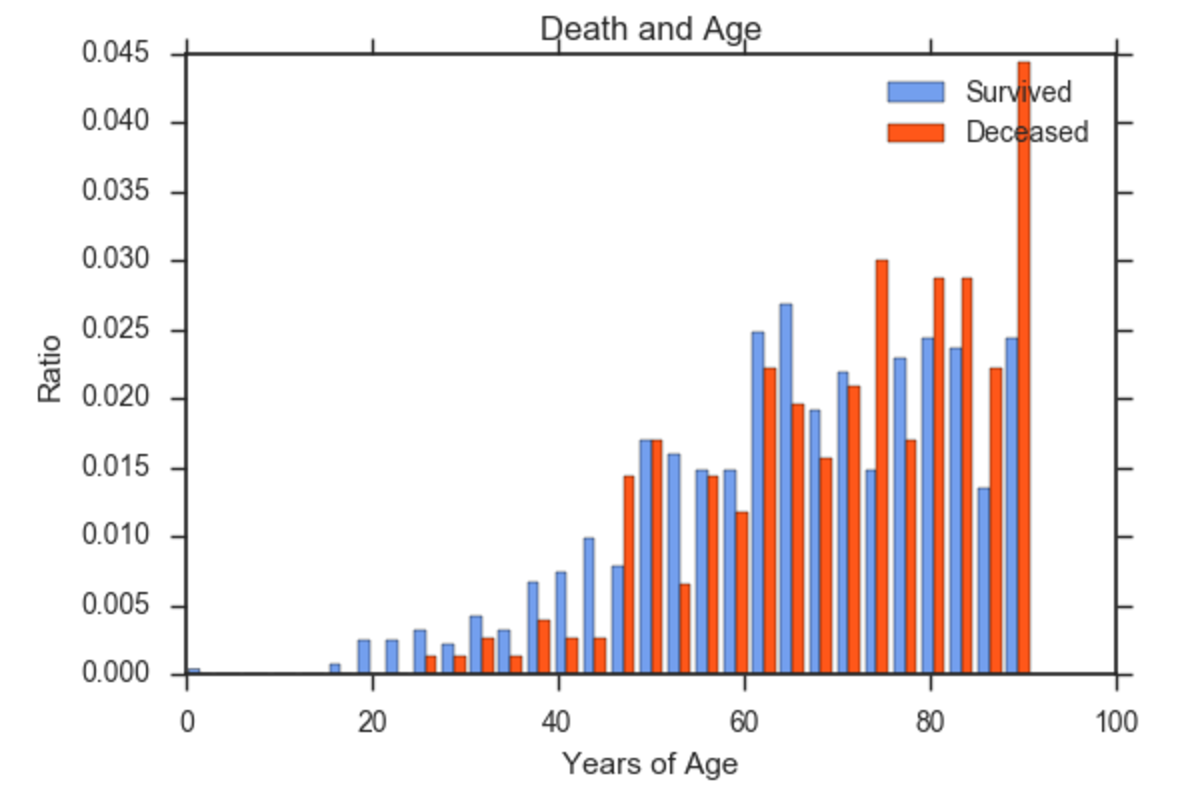
\includegraphics[width=0.48\textwidth]{age.png}
		\end{center}
		\caption{Age Breakdown}
	\end{wrapfigure}
	
	There is a somewhat noticeable trend in \textbf{figure 1} with regards to age and survivability of sepsis but it doesn't appear to be anything that an algorithm could rely on strongly. It is important to discover some other useful features.
	
	It may be useful to look at the initial blood tests for feature correlation. Observing all of these blood tests that are correlated with sepsis, the following were had enough datapoints to be useful: bicarbonate, INR, MCH, AST, alkaline phosphatase, PH, creatinine, platelet, PT, PTT, lymphocytes, RBCDW, calcium, neutrophils, glucose, hematocrit, hemoglobin, lactate, BUN, age.
	
	Looking at the feature correlation in \textbf{figure 2} gives a better understanding of how the features are correlated with one another as well as which features have a strong or negative correlation to the survivability of sepsis.
	
	
	
	
	There appear to be a few values with very strong correlation such as PTT and INR. PTT, PT, and INR are all used to test for clotting factors in blood so this result is logical. This also means that these features could probably be compressed into fewer dimensions.
	
	\begin{wrapfigure}{l}{0.70\textwidth}
		\begin{center}
			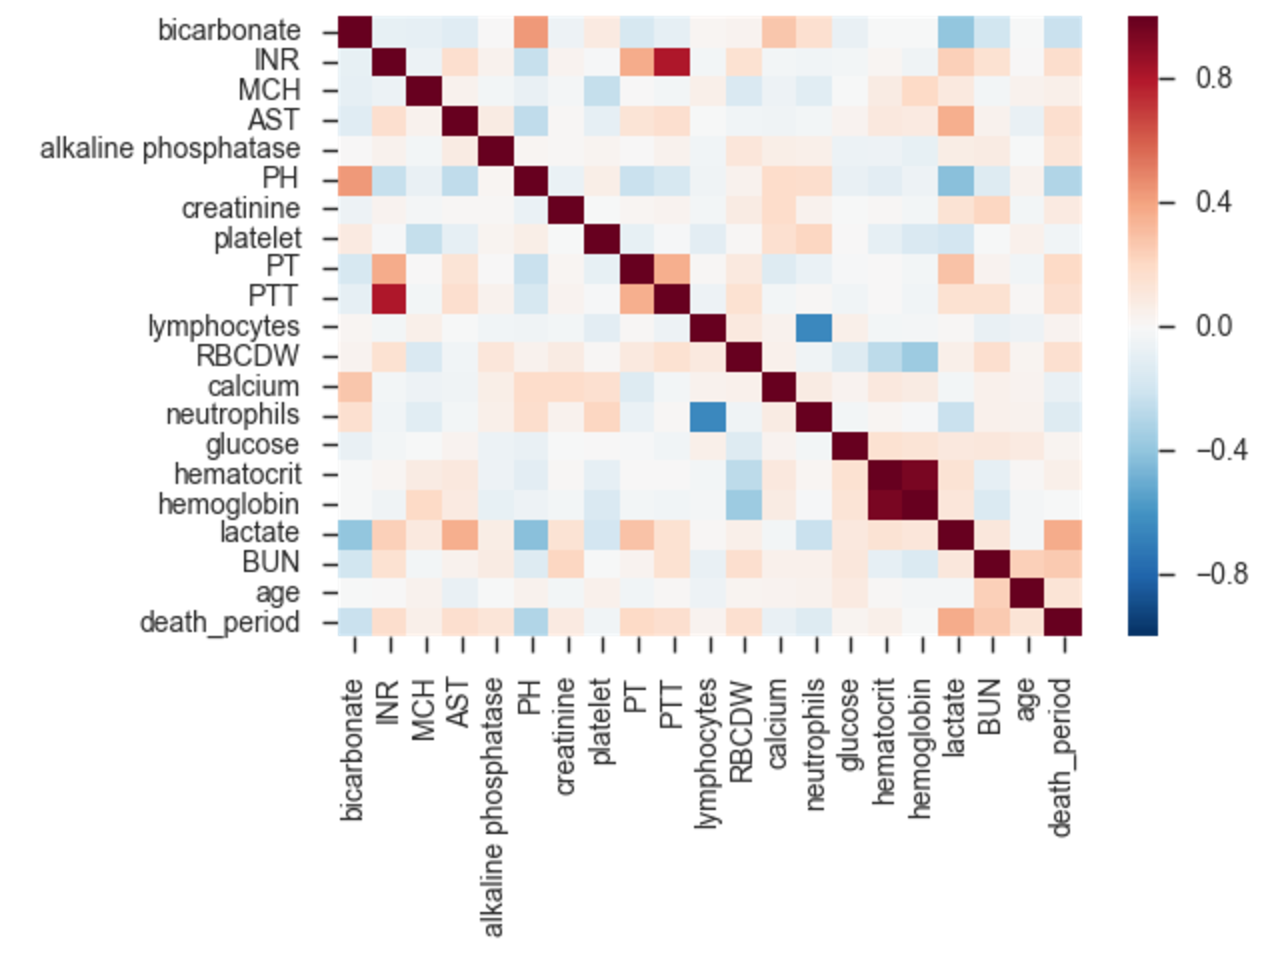
\includegraphics[width=0.68\textwidth]{feature_correlation.png}
		\end{center}
		\caption{Patient Vitals Correlation}
	\end{wrapfigure}
	
	Within the 30 day period of mortality, there are none with a positive or negative correlation over +/-0.4 however there are some useful features to consider. Lactate is relatively strongly correlated with ~0.38 with blood urea nitrogen(BUN), and PH not far behind. Lactate is an indication of shock, since lactate is produced by cells that are note receiving enough oxygen. PH is a byproduct of the acidic lactate in the patients blood hence the correlation. Blood urea nitrogen is an indication that the kidneys are failing to process the excess urea in the blood. This can indicate potential kidney damage or failure. All of these are much more useful than age, which is a good sign for our ability to predict.
	
	\begin{wrapfigure}{r}{0.50\textwidth}
		\begin{center}
			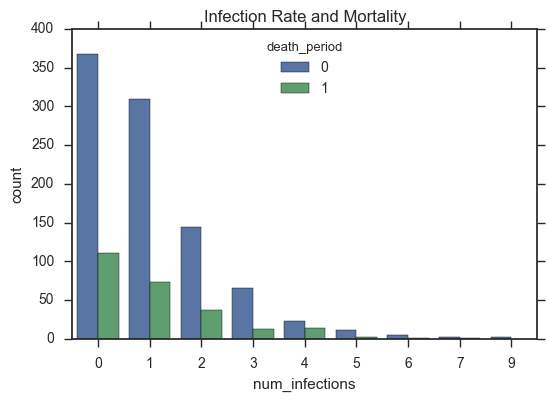
\includegraphics[width=0.48\textwidth]{bio_graph.png}
		\end{center}
		\caption{Infection Count and Mortality}
	\end{wrapfigure}
	
	Finally considering microbiology events. Every infection type is taken and the correlation considered. Though the assumption might be made that infection is strongly correlated with the survivability of sepsis, it is important to note that once a patient is septic, the infection type plays little role. Let us look at number of infections and survivability in \textbf{figure 3}.
	
	There appears to be very little correlation after further observation between survivability and number of infections. With the majority of patients not having an infection discovered within the first 24 hours. Due to this lack of information, the infection type is likely not useful. 
	
	These visualizations give some useful insights into the data. One of these insights is that there is nothing that strongly indicates a patient will or will not survive sepsis. Many independent features must be taken into consideration and trends found. Due to this nature of the data, a neural network, or an ensemble technique like adaptive boosting or extreme gradient boosting may prove useful. 
	
	
	
	\subsection{Algorithms and Techniques}
	Four different classifiers will be compared for their accuracy score. These classifiers are the following:
	
	\begin{enumerate}
		
		\item \textbf{Support Vector Machine:} Support vector machines are a flexible yet simple machine learning algorithm. When compared to a neural network, SVMs require much less grid-searching to optimize hyperparameters. SVMs can approximate complex non-linear functions with the "kernel trick". This is useful considering the nature of this dataset. SVMs are also guaranteed to find the global optima, not just local like some machine learning algorithms.
		
		Support vector machines like neural networks are a black box. It is hard to interpret the model once it has been created. SVMs can also suffer from too many training examples, bloating the time it takes to train. This potential issue will not be a problem with this relatively small dataset however.
		
		\item \textbf{Adaptive Boosting:} Adaboost is another fantastic ensemble method. It is notorious for not overfitting to data. It is quite flexble due to its ability to leverage any base estimator works best in a certain situation. Adaboost itself has few parameters to tweak to increase performance so it works relatively well right out of the box.
		
		While Adaboost is one of my favorite algorithms so far, it does have some pretty strong weaknesses. It is most often always not the best in class predictor. There typically are more accurate classifier options on the table. It is also sensitive to noisy data as well as outliers. This is similar to Random Forests. The reason I included both of these ensemble techniques is because I wanted to compare their output to classifiers known to be better at handling noisy data. These are great classifiers but are unlikely to be the most accurate.
		
		\item \textbf{Neural Network:} Neural networks are an incredibly powerful machine learning algorithm. They can approximate any nonlinear function, highly customizable, and robust to outliers. With these features, it is possible to create a highly accurate predictor of the data but it is important to take into consideration the weaknesses of neural networks as well.
		
		Neural networks, while powerful, have some pretty strong weaknesses. They are difficult to set up and difficult to tune because of the number of parameters. It is also necessary to decide on the architecture of the network yourself. It is not nearly as simple to set up as the previous examples. It is also quite easy to overfit data using neural networks. Without restraint they have a strong affinity to fit to noise in the data. Due to the nature of this dataset it will be a important task to keep this algorithm in reign to prevent overfitting.
		
		\item \textbf{Extreme Gradient Boosting} XGBoost is an optimized distributed gradient boosting library. Gradient boosting in general is thought of as one of as one of as a best in class predictor. It can approximate most nonlinear functions, and automatically handles missing values. This is a very powerful algorithm that is much less work to set up than a neural network.
		
		Gradient boosting can overfit if run for too many iterations and can be sensitive to noisy data or outliers. This is an unfortunate downside but it is common in many algorithms. It will be important to preprocess the data to remove outliers.
	\end{enumerate}
	
	These are relatively varied algorithms with much different predictive techniques. The comparison between the predictive accuracy will allow some insight into how the algorithms behave with moderately small datasets with a natural noise and outliers. It is a considerable task to preprocess the data properly in order to optimize the results.
	
	\subsection{Benchmark}
	There are few studies into the predictability of patient survival from severe sepsis. There are also many factors that are important in how the prediction is made. I will be focusing on the following research: ``Predicting survival of patients with sepsis by use of regression and neural network models'' by J.R. Flanagan, et al. 
	\begin{quotation}
		``Survival after sepsis was predicted with an accuracy of 80\% by the NN model, which used only information collected at the time of the diagnosis of sepsis. The development of multiple organ failure after the diagnosis of sepsis was predicted accurately (81.5\%) with either the MLR or the NN model. Both the MLR and the NN methods depended on the interpretation of a likelihood quantity, requiring the choice of a threshold to make a survival prediction. ''\cite{sepsisresearch}
	\end{quotation}
	
	While this study was done in 1996, there have been few follow-up studies. The few follow-up studies had a similar success rate with slightly different attributes and test periods. Due to the detail of this study, most focus will be put on the work of Flanagan et al. for the benchmark.
	
	In the analysis I am conducting, patients are admitted with suspected sepsis and all vitals and lab tests within 24 hours of admission are used in the classification task. This is to standardize periods of importance across all patients observed.
	
	\section{Methodology}
	\subsection{Data Preprocessing}
	Preprocessing the data is the most challenging and time consuming step of this process. All pre-processing and visualization was initially done in the Jupyter notebook titled \textbf{Septic Feature Probe.ipynb} and later all preprocessing is done again the in the final model comparison analysis in the Jupyter notebook titled \textbf{Sepsis Model Comparison.ipynb} along with the helper python file \textbf{mimicpreprocess.py}. The following steps were taken to preprocess the data:
	
		\subsubsection{Acquire the Dataset}
		The MIMIC-III dataset is openly available and developed by the MIT Lab for Computational Physiology. It first requires certification to handle de-identified medical information. The data is provided in CSV files, with each file representing a table in a database. The CSVs were then processed and imported into respective tables in a PostgreSQL database.
		
		An exhaustive search of all potentially useful features was done by mapping and searching the database using the DBVisualizer application. Most features were not feasible for use do to lack of associated date-time information. Four tables were found to have all necessary information to link data to an individual patient, an individual patient's stay, and consider information gained within the first 24 hours from admission. These tables were related to:
		
		\begin{enumerate}
			\item \textbf{Admission Information:} This table included the patients ethnicity, language, insurance type, admission date, suspected diagnosis, and discharge information
			
			\item \textbf{Patient Data:} This table is more of a "through table" with the patient's ID, date of birth, gender, and date of death (if applicable).
			
			\item \textbf{Lab Test Results:} This table is extensive and contains all test results associated with each patient. Lab tests are identified with an ID (eg: 50912 is results for blood creatinine tests), a numeric result, a unit, and a date-time. Several correlational studies were read to identify lab tests that provide insight into the stage of sepsis. Some of these included: Creatinine, blood ph, dissolved Co2, lactate levels etc. These features were acquired and explored further. 
			
			\item \textbf{Microbiology Results:} This table contains all microbiology lab results. It indicates the type of infection, the date-time for the test, and resulting treatment.
			
		\end{enumerate}
	
		The multiple other tables were unusable for the most part due to lack of uniform data capturing between MetaVision and CareVue origin systems. 
		
		With the data identified and obtainable, the next step was to import data into a usable format in python utilizing the SQLAlchemy python library.

		\subsubsection{Calculate Features}
		It was required to calculate most features due to the nature of the database and of medical data in general. Missing values also need to be dealt with properly. The following was done to calculate the feature set:
		
		\begin{enumerate}
			\item For all potentially useful lab results the mean value was taken along with the maximum and minimum measurements as separate features.
			\item Age was calculated from DOB and Admission date. For patients over 89 the median age of 93 was taken due to HIPAA constraints.
			\item For each patient, infection types and infection count were taken as separate features. Each infection type was it's own binary feature.
			\item Prior hospital stays was calculated by looking at admission date and subject\_id to see if the patient had been to the hospital in this previous timespan.
			\item A binary death period value was calculated. This feature represented whether a patient expired within 30 days of hospital admission. Only deaths that are related to sepsis are of interest for this study. 30 days is a standard period to observe.
		\end{enumerate}
	
		\subsubsection{Handle Missing Values and Outliers}
	
		Many patients had missing vital measurements. If approximately 15\% of the patients were missing values for a single feature, the feature was dropped. This was done to prevent any machine learning algorithm fitting to false or replaced values.
		
		Patients that were missing approximately 30\% of the selected lab results were dropped due to the lack of information. These patients may have been admitted and discharged quickly or an error in recording could have occurred.
		
		Medical information is irregular which resulted in most patients missing information from at least one feature. To handle this, the mean value from the entire feature set was taken and filled into this cell. There are many techniques to handle filling in missing information however, taking the median tends to work quite well and is simple to implement.
		
		Potential outliers were calculated and removed. First a step was calculated: \(step = 1.5*(Q3-Q1)\). If the feature was less than the first quartile minus the step (\(Q1 - step\)) or greater than the third quartile plus the step(\(Q3 + step\)), it was considered a column outlier. If an entry had greater than 4 column outliers, it was removed.
		
		\subsubsection{Standardizing Features}
		Now the data is more or less usable but each column contains multi-categorical data or numerical data in different units.
		
		Categorical data is converted into one-hot features where each category has its own column with it on or off. This task is made easy with Pandas' built in functionality of \(pandas.get\_dummies(df)\).
		
		Certain machine learning algorithms might behave poorly if individual features do not more or less look like standard normally distributed data. A feature that is naturally much higher could smother the naturally smaller values in the prediction. This is not always the case but it is a good idea to standardize all data to prevent such an error. This moves the mean to zero. The operation is easily done by fitting data to \(sklearn.preprocessing.StandardScaler()\).
		
		\subsubsection{Feature Selection}
		There are many features that may be of little use when predicting the survivability of sepsis. The more irrelevant features that exist, the more data is required to ensure they do not fit to noise in those features. It is important to remove the features that are of little use. 
		
		\begin{wrapfigure}{l}{0.50\textwidth}
			\begin{center}
				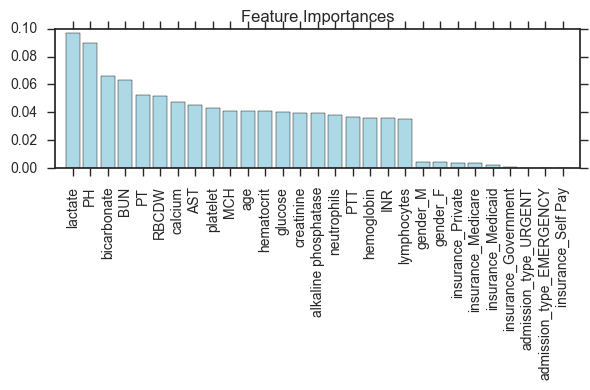
\includegraphics[width=0.48\textwidth]{feature_correlation_2.png}
			\end{center}
			\caption{Feature Correlation Graph}
		\end{wrapfigure}
		
		Feature correlation was calculated and it was observed that the infection type was of little correlation to the survivability of sepsis. The existence of any infection was of little use in predicting survivability as well, therefore these features were dropped from the dataset.
		
		With the remaining features, a random forest was trained and the resulting feature importances graphed in \textbf{figure 4}.
		
	
		As can be seen in \textbf{figure 4}, gender, insurance type, and admission type are of little use when predicting survivability. For most algorithms, this data will be dropped. For the neural network, it may be included since more complex relationships could be developed between the features.
	
		The important features have been discovered and now machine learning models can be trained on this cleaned and standardized data.
	
	\subsection{Implementation}
	Four different machine learning algorithms were implemented and trained therefor four different processes were required to develop them. All work can be seen in the Jupyter notebook titled \textbf{Sepsis Model Comparison.ipynb} along with the helper python file \textbf{mimicpreprocess.py}. Prior to any models developed, the data must be loaded into a pandas dataframe and preprocessed as described in the previous section.
	
	\subsubsection{Support Vector Machine}
		Most of the SciKitLearn machine learning algorithms tend to be quite easy to set up and run, much more so than XGBoost or a Neural Network. SVMs should, in theory, work great with this dataset due to its size and complexity. The process is as follows:
		
	\begin{enumerate}
		\item \textbf{Define Model:} A model is defined with a random state in order to reproduce the results and the type of kernel, \textbf{rbf}.
		\item \textbf{Define Parameters:} A parameter grid defines several important hyperparameters to test. They are as follows:
		\begin{enumerate}
			\item \textbf{C:} The C hyperparameter controls the smoothness of the decision boundary by telling the SVM  how much you want to avoid misclassification. Large C will cause the optimizer to find a larger margin separating the hyperplane while small C will result in a larger margin separating the hyperplane at the expense of misclassifying points.
			\item \textbf{gamma:} gamma controls how many support vectors are used in placing said decision boundary. When gamma is very small, the model can be too constrained and is unable to capture the complexity of the data. However if gamma is too high, the model will fit to noise to few support vectors.
		\end{enumerate}
		\item \textbf{Grid Search:} Due to the size of the hyperparameter test set, GridSearchCV is used to iterate over every possible combination of parameters in the param\_grid. Note that \textbf{stratified k-fold} cross validation is used with 10 folds total. 
	\end{enumerate}	

	\subsubsection{Adaptive Boosting}
		The AdaBoost model implementation is as follows:
		\begin{enumerate}
			\item \textbf{Define a Base Estimator:} The base estimator is what AdaBoost boosts. It is a very important selection. In order to make the algorithm generalizable and prevent overfitting, a decision stump (1d decision tree) is selected and defined as the base estimator.
			\item \textbf{Define Model:} A model is defined with a random state in order to reproduce the results and the decision stump as the base estimator.
			\item \textbf{Define Parameters:} The adaboost parameter grid is defined as follows: 
			\begin{enumerate}
				\item  \textbf{n\_estimators:} n\_estimators controls the max number of estimators at which boosting is terminated. The more estimators, the more complex the model, so it is important to look for a reasonable number and signs of overfitting.
				\item \textbf{learning\_rate:} The learning rate shrinks the contribution of each classifier. If the learning rate is too large, the optimal solution can be missed. If too small, too many iterations may be required. There is a tradeoff between the number of estimators and the learning rate.
			\end{enumerate}
			\item \textbf{Random Search:} Due to the size of the hyperparameter test set, RandomSearchCV is used to iterate randomly over the possible combinations of parameters in the param\_grid. Note that \textbf{stratified k-fold} cross validation is used with 10 folds total. Random search is used here instead of grid search since the number of hyperparameters that are tested is much larger and in practice works nearly as well with a reasonable number of iterations. In this case 100 iterations were done.
		\end{enumerate}	
	
	While Adaboost may seem like a relatively complex algorithm, the most complex task is selecting a solid base estimator. There are few hyperparameters to tune and better performance comes from manipulating the data to work optimally with such an algorithm.
	
	\subsubsection{Extreme Gradient Boosting}
		Extreme gradient boosting is slightly more complex to implement than the previous models. The XGBoost python library will be used due to it's performance and community support. The model implementation is as follows:
		
		\begin{enumerate}
			\item \textbf{Define Model:} A model is defined with the \textbf{objective = binary:logistic}. binary:logistic is for binary classification, it returns predicted probability not the class.
			\item \textbf{Define Parameters:} There are more parameters to test in XGBoost than in the previous algorithms, they are as follows:
			\begin{enumerate}
				\item \textbf{max\_depth:} max\_depth represents the maximum depth of a tree. Higher values will lead to a more complex model but also has the potential to fit to noise in the dataset. A typical value is between 3 and 10.
				
				This value can have large ramifications since XGBoost makes splits upto the max\_depth then start pruning the tree backwards and remove splits which there is no positive gain.
				\item \textbf{gamma:} gamma represents the minimum loss reduction required to further partition on a leaf node. The larger the value, the more conservative the algorithm. 
				
				It is important to note that the values of gamma can vary depending on the loss function and therefore should be tuned.
				\item \textbf{min\_child\_weight:} min\_child\_weight is the minimum sum of instance weight required in a child node. If a tree partition step results in a child weight less than the minimum, the building process will halt further partitioning. 
				
				The minimum child weight has high impacts on the model outcome and therefore must be heavily tuned.
				\item \textbf{n\_estimators:} n\_estimators represents the number of trees to be boosted by the XGBoost model. More trees can increase complexity and potential for overfitting so ensuring a reasonable value is tuned is important.
				\item \textbf{learning\_rate:} The learning\_rate or eta is the step size shrinkage used in update to prevents overfitting. After each boosting step the eta will shrink the feature weights to make the algorithm more conservative and reduce the likelyhood of overfitting. 
			\end{enumerate}
			\item \textbf{Randomized Search:} Due to the size of the hyperparameter test set, RandomizedSearchCV is used to iterate over randomly the possible combinations of parameters in the param\_grid. Note that \textbf{stratified k-fold} cross validation is used with 10 folds total. 
	\end{enumerate}

	It can be seen that many of the hyperparameters that are tuned have significant interaction and play between one another. XGBoost provides many "knobs" to increase and decrease model complexity while allowing granular selections to reduce the probability of overfitting. XGBoost is complex and quite powerful due to this flexibility.
	
	\subsubsection{Neural Network}
	
	\begin{wrapfigure}{r}{0.50\textwidth}
		\begin{center}
			\includegraphics[width=0.48\textwidth]{diagram.png}
		\end{center}
		\caption{Keras Neural Network Flow}
	\end{wrapfigure}

	An artificial neural network is the most complex machine learning algorithm that is used in this project. Much of its flexibility is due the fact that the general architecture must be designed instead of simple hyperparameter tuning and data manipulation. To design a NN, the following steps were taken:
	
	\begin{enumerate}
		\item Define the basic network architecture
		\item Define and test hyperparameters with dataset. These included:
			\begin{enumerate}
				\item Number of neurons per layer.
				\item Activation function per layer.
				\item The kernel constraint per layer. Used to reduce the probability of overfitting.
				\item Dropout ratio per layer. 
				\item Batch size.
				\item Number of epochs to observe results over.
			\end{enumerate}
		\item Define the loss and accuracy funtion.
		\item Train the network and log per-epoch loss and accuracy score.
		\item Plot logged accuracy and loss scores.
		\item If accuracy and/or loss is unacceptable return to the start, considering manipulated existing data by adding or removing features.
	\end{enumerate}
		


	\textbf{Figure 5} illustrates the general architecture of the neural network that was used on this dataset. The number of iterations through this graph is controlled by the batch size and the number of epochs. Smaller batch sizes requires more iterations to see the entire dataset.
	
	The acronyms and nodes on the graph are as follows:
	\begin{enumerate}
		\item \textbf{DL:} DL represents a densely connected layer. Each neuron is connected to all other neurons.
		\item \textbf{DOL:} DOL represents a drop out layer. Drop out layers are used to reduce data memorization/overfitting by randomly removing a portion of the neurons which causes the other neurons to react to this loss. Having a drop out layer is useful when the size of the dataset is relatively small.
		\item \textbf{epoch:}  An epoch is a single pass through the entire training set which is then followed by the testing set.
		\item \textbf{loss:} A loss function is calculated using the desired and actual output of the network. The loss function will return an error value for each of the neurons in the output layer. Many different loss functions can be used but in this case, binary cross entropy is used.
	\end{enumerate}

	\subsection{Refinement}
	As mentioned in the Benchmark section, 80\% accuracy was achieved by J.R. Flanagan, et al. using a Neural Network model. The results from all of the machine learning algorithms will be compared to this result for refinement.
	
	The initial pass of the data through each of the algorithms was the following:
	
	\subsubsection{SVM}
	The initial classification accuracy of the trained support vector machine was \textbf{79.2\%}. This is already relatively close to the benchmark previously discussed.
	
	At this point the dataset contained the mean vital readings as well as maximum and minimum readings, removing the maximum and minimum readings was the first step to reduce dimensionality and potentially increase performance. The next step was to grid search even more \textbf{gamma} and \textbf{C} values. After these optimizations, the performance of the SVM increased to \textbf{81.8\%} accuracy.
	
	\subsubsection{Adaptive Boosting}
	The initial classification accuracy of AdaBoost was \textbf{80.0\%}, exactly the benchmark. This was a surprising result but performance could be improved.
	
	The same was done as with the SVM, where the max and min values were trimmed from the dataset. The decision stump base estimator was also swapped out for the default estimator which is a standard decision tree. This resulted in an increase in accuracy to \textbf{82.3\%}. 
	
	\subsubsection{Extreme Gradient Boosting}
	The initial classification accuracy of XGBoost was \textbf{80.2\%} slightly above the benchmark. This is quite a good result without manipulating the existing data or more hyperparameter tuning.
	
	The max and min patient vital features appeared to be affecting XGBoost negatively, the same as Adaboost or SVM. None performed better with dimensionality reduction as well. The max and min values were dropped. The range of the hyperparameters being tested was widened and min\_child\_weight was added for testing instead of using the default value. These changes resulted in an increased accuracy score to \textbf{82.6\%}. 
	
	\subsubsection{Neural Network}
	The initial classification accuracy of the Keras Neural network using Tensor Flow was not impressive at \textbf{70.2\%}. The initial Neural network was much simpler than the final version discussed in detail in the previous section. The initial NN had no dropout layers, no kernel constraint parameter, had only 1 hidden layer and had very few neurons per layer at 10.
	
	In the final version, 3 hidden layers are present, dropout layers were added, a kernel constraint was added, additional data features were considered including gender, the number of nodes were iteratively increased and decreased per layer resulting in a much more robust model. This resulted in an increased accuracy at \textbf{85.8\%} on the 77-80th epoch. This is quite an impressive score compared to the benchmark and other models tested here.
	
	It is important to note that this accuracy was selected from the optimal section of hundreds of epochs. Due to the nature of machine learning algorithms each running resulted in different accuracy scores.
	
	\bibliography{citations}{}
	\bibliographystyle{ieeetr}
	
\end{document}